\documentclass{article}
\usepackage[utf8]{inputenc}
\usepackage{geometry}
\usepackage[T1]{fontenc}
\usepackage{amsfonts}
\usepackage{amsmath}
\usepackage{amssymb}
\usepackage{graphicx}
\usepackage{float}
\usepackage{hyperref}
\usepackage[sorting=none]{biblatex}
\usepackage{fancyhdr}
\usepackage{multicol}
\usepackage{enumitem}
\usepackage{tikz}
\usepackage{listings}
\lstset{
    basicstyle=\footnotesize\ttfamily,
    breaklines=true,
    keywordstyle=\bfseries\color{blue},
    commentstyle=\itshape\color{green!40!black},
    stringstyle=\color{orange},
    numbers=left,
    numberstyle=\tiny,
    stepnumber=1,
    tabsize=4,
    showstringspaces=false
}
\usepackage{bm}
\usetikzlibrary{shapes,arrows,fit,positioning}
\addbibresource{ref.bib}
\setlength{\columnsep}{40pt}
\setlength{\voffset}{0.7cm}
\setlength{\headsep}{40pt}
\geometry{legalpaper, portrait, margin=2cm}


% Title page
\title{HW B2: MEP Voting Patterns}
\author{Andrea Stanziale}
\date{\today}

% Header and footer
\pagestyle{fancy}
\fancyhead{}
\fancyhead[L]{\textbf{Machine Learning, Advanced Course}\\\textbf{DD2434}}
\fancyhead[R]{\textbf{Andrea Stanziale}\\ stanz@kth.se}
\fancyfoot{}
\begin{document}

\maketitle

\section{Data and Similarity Matrix}
% ------------------------------------------------------------

\subsection{Data Description}

We have a dataset containing MEP votes, with columns such as:
\begin{itemize}
    \item \texttt{MEP\_ID}, \texttt{Country}, \texttt{EPG}, \ldots
    \item Several columns of numeric codes for votes (e.g., 1 = For, 2 = Against, 3 = Abstention, 4 = Absent, 5 = Didn't Vote).
\end{itemize}

Each MEP is associated with an entire vector of votes. We encode those as:
\[
    \text{Yes} \to +1,\quad 
    \text{No} \to -1,\quad
    \text{Abstain} \to 0,\quad
    \text{Absent / Missing} \to \text{NaN}.
\]

\subsection{Similarity Computation}

We compute a pairwise similarity, via \emph{cosine similarity}:
\[
    \text{Sim}(\mathbf{v}_i, \mathbf{v}_j)
    = \frac{\mathbf{v}_i \cdot \mathbf{v}_j}{\|\mathbf{v}_i\|\|\mathbf{v}_j\|}.
\]
The cosine similarity is a good similarity measure in this context, as it is invariant to the length of the vectors and only depends on the angle between them.
Furthermore, compared to other similarity measures such as the \emph{agreement rate}:
\[
    \text{Sim}(\mathbf{v}_i, \mathbf{v}_j) 
    \;=\; \frac{\sum_{k \in K_{ij}} \mathbf{1}[v_{i,k} = v_{j,k}]}{|K_{ij}|},
\]
rewards "closer" votes, so for example a "no" vote is considered closer to abstaining than it is to a "yes" vote.
After computing the \(N\times N\) similarity matrix \(\mathbf{S}\), we aim to transform it into a distance matrix \(\mathbf{D}\).

% ------------------------------------------------------------
\section{Classical MDS}
% ------------------------------------------------------------

\subsection{Distance Matrix Construction}

Since classical MDS (Torgerson MDS) typically uses a distance matrix \(\mathbf{D}\), we define:
\[
       D_{ij} \;=\; \sqrt{1 - S_{ij}}
\]
provided \(0 \le S_{ij} \le 1\). That gives us an \emph{approximate} distance in \([0,\sqrt{1}]\). 

\subsection{Classical MDS Steps}

Let \(\mathbf{D}\) be the \(N \times N\) distance matrix with entries \(D_{ij}\). The classical MDS algorithm is:

\begin{enumerate}
    \item Compute the matrix of squared distances: \(\mathbf{D}^{(2)}\) where \(\mathbf{D}^{(2)}_{ij} = D_{ij}^2.\)
    \item Define the centering matrix 
    \[
        \mathbf{H} \;=\; \mathbf{I}_N - \frac{1}{N} \mathbf{1}_N \mathbf{1}_N^T,
    \]
    where \(\mathbf{1}_N\) is the \(N\)-vector of all ones.
    \item Form 
    \[
        \mathbf{B} \;=\; -\tfrac12 \, \mathbf{H} \,\mathbf{D}^{(2)}\, \mathbf{H}.
    \]
    \item Perform an eigen-decomposition of \(\mathbf{B}\):
    \[
        \mathbf{B} = \mathbf{V}\,\mathbf{\Lambda}\,\mathbf{V}^T,
    \]
    where \(\mathbf{\Lambda}\) is the diagonal of eigenvalues \(\lambda_1 \ge \lambda_2 \ge \cdots \ge 0\).
    \item Pick the top \(r\) components (for 2D, \(r=2\)) to define
    \[
        \mathbf{X}_r = \mathbf{V}_r \, \mathbf{\Lambda}_r^{1/2}.
    \]
    Each row of \(\mathbf{X}_r\) is a point in \(\mathbb{R}^r\) representing an MEP.
\end{enumerate}



% ------------------------------------------------------------
\section{Results and Plots}
% ------------------------------------------------------------

Having computed \(\mathbf{X}_2\) of size \(N \times 2\), we can plot these 2D coordinates in a scatterplot.

\subsection{Plot by EPG}

We color each MEP by their political group (EPG).  The results are displayed in \autoref{fig:epg_plot}.
We notice a clear clustering by EPG, suggesting that party affiliation is a strong factor in determining voting similarity.
We notice that some groups tend to vote less similarly to others, these groups are normally groups at the extremes of the political spectrum (The LEFT, NI, ECR).

\begin{figure}
    \centering
    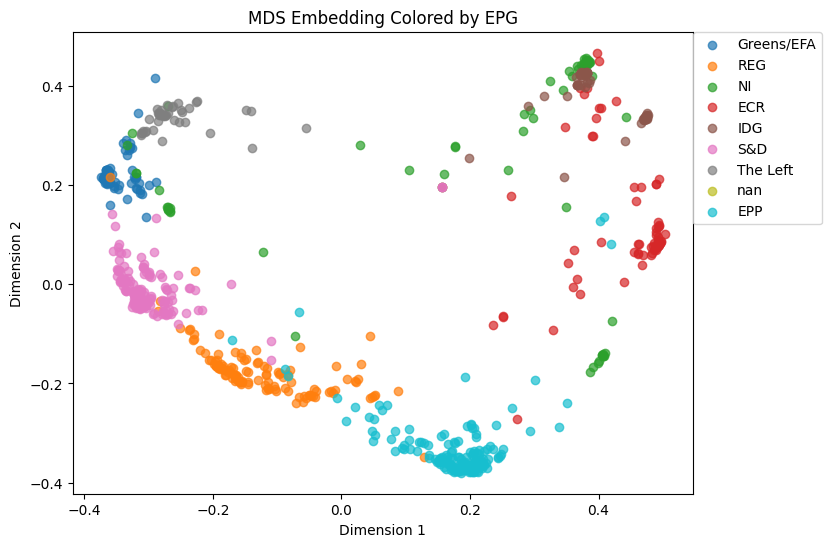
\includegraphics[width=0.7\textwidth]{MDS_EPG.png}
    \caption{MDS Embedding Colored by EPG}
    \label{fig:epg_plot}
\end{figure}

\subsection{Plot by Country}

Similarly, we color by country. The results are displayed in \autoref{fig:country_plot}. As expected, the country affiliation is a less strong predictor of similarity than party affiliation. 
We see that MEPs from the same country are often spread out in multiple clusters, likely determined by the party of the MEPs taken into consideration.
\begin{figure}
    \centering
    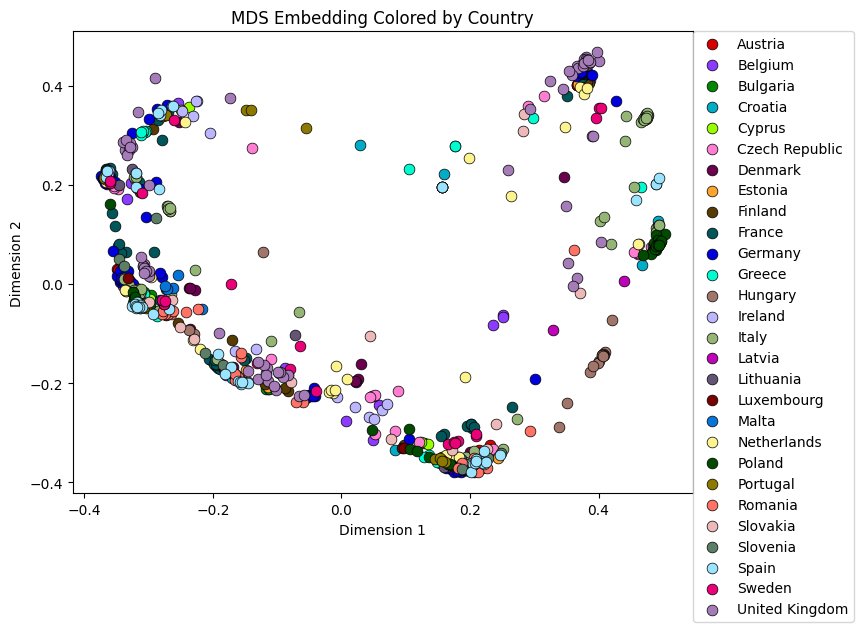
\includegraphics[width=0.7\textwidth]{MDS_Country.png}
    \caption{MDS Embedding Colored by Country}
    \label{fig:country_plot}
\end{figure}

% ------------------------------------------------------------
\section{Hierarchical Clustering}

In this section, we apply hierarchical clustering to our distance matrix of MEPs. The motivation for choosing hierarchical clustering over alternative methods (such as K-means) is twofold: 
\begin{enumerate}
    \item \textbf{Flexibility in the number of clusters:} Hierarchical clustering does not require us to fix the number of clusters \emph{a priori}. Instead, we build a dendrogram that can be cut at different levels to reveal a hierarchy of possible partitions.
    \item \textbf{Interpretability:} The resulting dendrogram visually represents how MEPs (and subgroups of MEPs) merge step-by-step, which can be especially useful to observe potential alliances or subgroups that do not strictly correspond to official EPG or country divisions.
\end{enumerate}

\subsection{Ward's Linkage}

We take our $N \times N$ distance matrix, computed from the voting-based similarity scores, and convert it to a condensed distance format. We then use \textit{Ward's linkage} (or another chosen method) to iteratively merge the closest clusters. The resulting dendrogram is plotted with MEP labels on one axis, enabling us to examine at which distance threshold groups form or merge. The algorithmic steps can be summarized as follows:

\begin{itemize}
    \item \textbf{Initialization:} Each MEP starts in its own cluster.
    \item \textbf{Merging Steps:} At each iteration, the two clusters with the smallest inter-cluster distance are merged into a new, larger cluster.
    \item \textbf{Dendrogram Construction:} We record the merges in a tree-like structure (the dendrogram), which illustrates how and when clusters coalesce.
\end{itemize}

\subsection{Results and Discussion}

Figure~\ref{fig:dendrogram} shows the hierarchical clustering dendrogram. Given the high number of entries, the dendrogram
is not immediately clear, so we also reported the findings in \autoref{tab:hiercluster}, by choosing 6 clusters. We see several interesting patterns:
\begin{itemize}
    \item Certain EPGs (e.g., S\&D) remain relatively cohesive, forming a single branch that merges with other branches only at higher distances.
    \item Other EPG (e.g., ECR, NI) splits into multiple sub-branches, suggesting internal diversity in voting patterns.
    \item Some MEPs from different EPGs cluster together at lower distances, indicating cross-party voting alignments.
\end{itemize}
These findings reveal that while official group membership generally corresponds to higher intra-group similarity, there are notable exceptions and hybrid clusters that do not align with the formal political groups.
Extending to different level of granularity can provide further insights into the MEP voting patterns and potential alliances across party lines.
For example, we analysed the distribution with two clusters to understand whether they align on the official government-opposition divide, or whether they form new alliances that are not immediately apparent from the official EPGs.
The results are summarized in \autoref{tab:epg-clusters}. It is interesting that the majority was split into two different clusters. The two clusters largely align into the left of center and right of center groups, while the majority coalition was formed by the EPP, S\&D, and REG groups. 

\begin{figure}[ht]
    \centering
    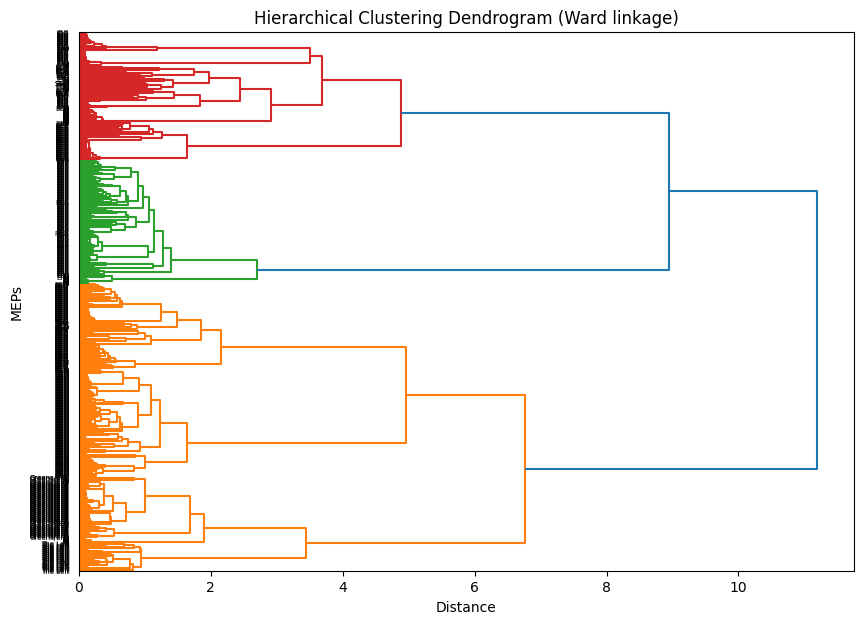
\includegraphics[width=0.8\textwidth]{dendrogram.png}
    \caption{Dendrogram illustrating hierarchical clustering of MEPs using Ward's linkage.}
    \label{fig:dendrogram}
\end{figure}

\begin{table}[ht]
  \centering
  \begin{tabular}{c|cccccccc}
       \textbf{Cluster} & \textbf{Greens/EFA} & \textbf{The Left} & \textbf{S\&D} & \textbf{EPP} & \textbf{ECR} & \textbf{IDG} & \textbf{NI} & \textbf{REG} \\
       \hline
       1 & 86 & 40 & 0 & 0 & 0 & 0 & 14 & 1 \\
       2 & 0  & 0  & 161 & 0 & 0 & 0 & 0 & 1 \\
       3 & 0  & 0  & 2 & 4 & 0 & 0 & 1 & 121 \\
       4 & 0  & 0  & 0 & 173 & 1 & 0 & 12 & 1 \\
       5 & 0  & 0  & 0 & 1 & 54 & 0 & 0 & 0 \\
       6 & 0  & 0  & 2 & 5 & 20 & 65 & 42 & 0 \\
  \end{tabular}
  \caption{Distribution of EPGs within the six clusters obtained from hierarchical clustering. Each column represents a distinct EPG, and the counts show how many MEPs from each group belong to each cluster.}
  \label{tab:hiercluster}
\end{table}

\begin{table}[ht]
  \centering
  \begin{tabular}{c|cccccccc}
       \textbf{Cluster} & \textbf{Greens/EFA} & \textbf{The Left} & \textbf{S\&D} & \textbf{EPP} & \textbf{ECR} & \textbf{IDG} & \textbf{NI} & \textbf{REG} \\
       \hline
       1 & 86 & 40 & 163 & 4 & 0 & 0 & 15 & 123 \\
       2 & 0  & 0  & 2   & 179 & 75 & 65 & 54 & 1 \\
  \end{tabular}
  \caption{Distribution of EPGs within the two main clusters obtained from hierarchical clustering. Each column represents a distinct EPG, and the counts show how many MEPs from each group belong to each cluster.}
  \label{tab:epg-clusters}
\end{table}



\vfill
\appendix
\section{Code}
\lstinputlisting[language=Python]{../similarity.py}
\lstinputlisting[language=Python]{../MDS.py}
\lstinputlisting[language=Python]{../clusterimg.py}




\end{document}

